\problem{}
The processed image by the median filter is shown in Figure \ref{fig:p3a}.
The median filter is selected with the size of $3\times 3, 5\times 5, 7\times 7$.

And we could see that the median kernel with size $3 \times 3$ has the best performance in this case.\\
The kernel has the proper size that remove the salt and pepper noise.

From the result, we could see that all the median filter processed images eliminate the salt and pepper noise, but the kernel size $3 \times 3$ has the best performance. The kernel size $5 \times 5$ and $7 \times 7$ make the 
processed images much blur than the $3 \times 3$ kernel size as they have the too big filter size to make information losses.

\begin{figure}[htbp]
    \centering
	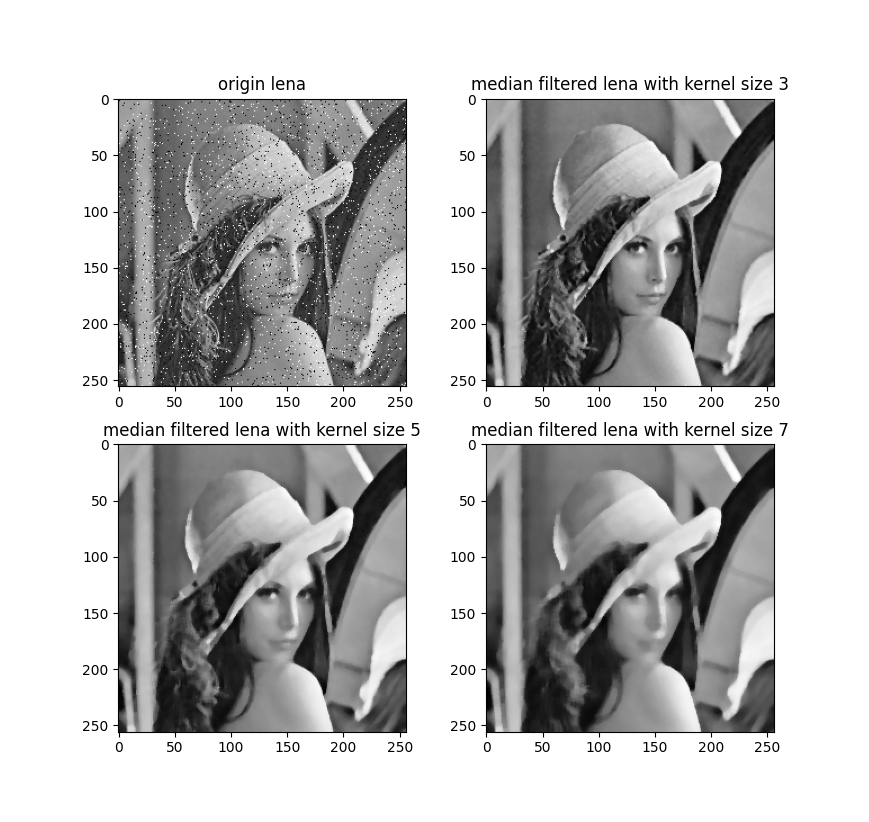
\includegraphics[width=\textwidth]{../images/p3/p3a.png}
    \caption{Median filter processed image}
\label{fig:p3a}
\end{figure}

The processed image by the and Gaussian filter is shown in Figure \ref{fig:p3b}.

Since the Gaussian filter's elements are $G(s,t)=Ke^{-\frac{s^2+t^2}{2\sigma^2}}$, but with the the normalize factor, the value of
$K$ would be eliminate, so $K$ does not matter. So we can just take $K=1$ and adjust the kernel size.

And we could see that no matter how the kernel size changes, the processed image is still blur than the median filter processed image. The Gaussian filter is not suitable for the salt and pepper noise removal.

\begin{figure}[htbp]
    \centering
	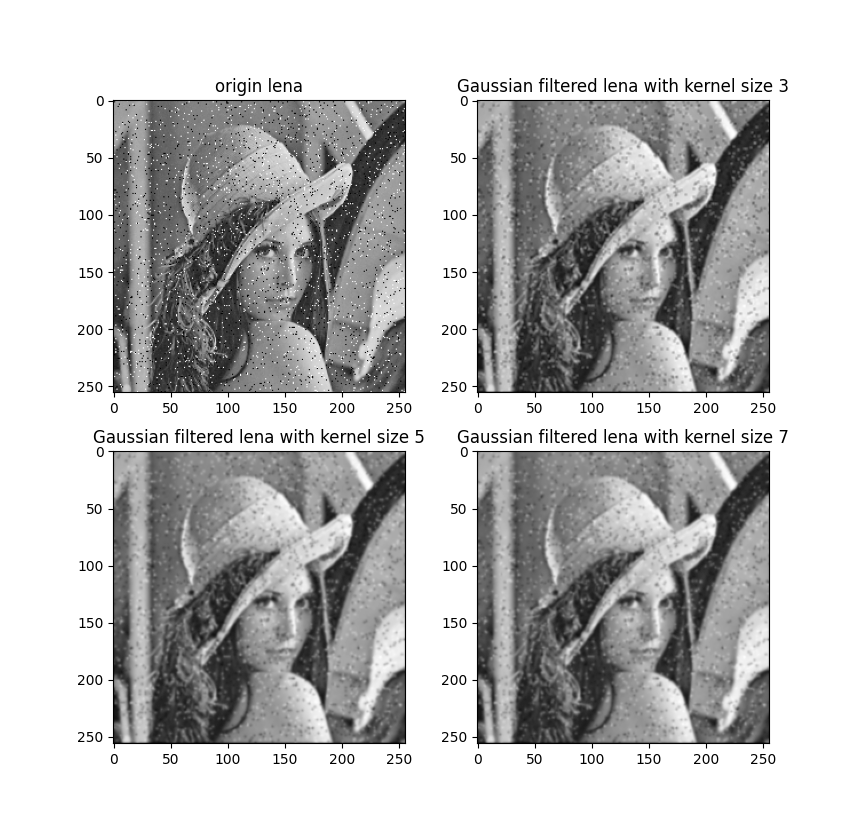
\includegraphics[width=\textwidth]{../images/p3/p3b.png}
    \caption{Gaussian filter processed image}
\label{fig:p3b}
\end{figure}

Analyse:\\
Salt-and-pepper noise is an impulse noise. It is extramly high($255$) or low($0$) pixel values.

Median Filter:\\
The median filter works by replacing each pixel value with the median value of all pixel in the patch. Since it is non-linear, it effectively removes noise. Since it replaces inpulse noise with the median value of the patch, it can perserve image's details and sharpness to recover the image from the noise.

The small-size filters ($3\times 3$) can remove the noise while perserving the sharpness and details of the image. But for the high density of noise, it may not be sufficient to remove the noise, but in our Lena's case, it removes noises sufficiently.

The large-size filters ($5\times 5$ or larger) may remove the high density of noise, but it may lead to the loss of image detail and make the image appear blurry.\\

Gaussian Filter:\\
The Gaussian filter is a linear smoothing filter that replaces each pixel value with a weighted average of the patch, the weights are normalized Gaussians. This gives the greatest weight to the central pixel, preserve the origin center's information sufficiently, and remove the noise by considering other pixels in the patch.
It works well on the Gaussian noises, but it does not work very well in our case's salt and pepper noise, as it is a linear filter, and weight the most to the center pixel, so it cannot remove the salt-and-pepper noise sufficiently, and cause the image blur.\\

The kernel size will effect the amplitude of each pixels' weights. With larger kernel, the amplitude of each part, especially for the center part becomes less, so it cause the result image smoother, and cause the salt-and-pepper noise not so obvious. 
But as the kernel size gets larger, the image also get much blurrer. From ours results, it seems that $5\times 5$ is better than the others, it somehow removes the salt-and-pepper noise, and make the image not too blur.\\

So above all:\\
Median filters are generally more suited for removing salt-and-pepper noise than Gaussian filters, especially when the noise density is high. And median filters also better preserve the sharpness and the recovery details.

The selection of kernel size should be case by case. Small kernel may not remove the noise sufficiently, while large kernel may cause the images loss the sharpness and details, cause the image blur. In this case, the $3\times 3$ median filter is the best.